\chapter{Context Enrichment Methods}\label{chap:context_enrichment_methods}
While in~\hyperref[chap:conceptual_architecture]{Chapter~\ref*{chap:conceptual_architecture}} the technical foundation for implementing the context enrichment methods was built, this chapter describes these on a more conceptual level. All approaches of context enrichment in this chapter do not rely on some pre-defined settings or data, instead they are applicable to general purpose ontologies as well as specialised ones of arbitrary size.

In this chapter, we present three context enrichment methods for ontology validation. While the first one, introduced in \hyperref[sec:neighboring_nodes]{Section~\ref*{sec:neighboring_nodes}}, takes neighbouring nodes~(i.e. subclass relations) into account, the second one, discussed in \hyperref[sec:embedded_context]{Section~\ref*{sec:embedded_context}}, is based on embedded context and the last one, explained in \hyperref[sec:external_source]{Section~\ref*{sec:external_source}}, uses external sources. 

\section{Neighbouring Nodes}\label{sec:neighboring_nodes}
This section starts with a conceptual overview of how neighbouring nodes in an ontology graph are used to generate contextual information. Then, existing approaches on generating textual definitions are examined. In the literature~\cite{soton265735} this task is also known under the term \textit{ontology verbalisation}. Even though that there exists \textit{OWL Verbalizer}\footnote{\url{http://mcs.open.ac.uk/nlg/SWAT/Verbaliser.html} accessed 2018/04/30}, a tool which already transforms generic ontologies into English sentences, we could not integrate it into the context enrichment process because 
\begin{inparaenum}[a)]
		\item it was designed as a standalone tool written in SWI-Prolog\footnote{\url{http://www.swi-prolog.org/} accessed 2018/04/30} and
		\item it only accepts the whole ontology as input
\end{inparaenum}.
However, in our approach we adopted some rules and integrated them in the enrichment process.

To illustrate the concept of neighbouring nodes and how they relate to the context enrichment approach explained later, a simple ontology graph describing the teacher/pupil domain is given in~\hyperref[fig:simple_owl_graph]{Figure~\ref*{fig:simple_owl_graph}}.
\begin{figure}
	 \centering
	 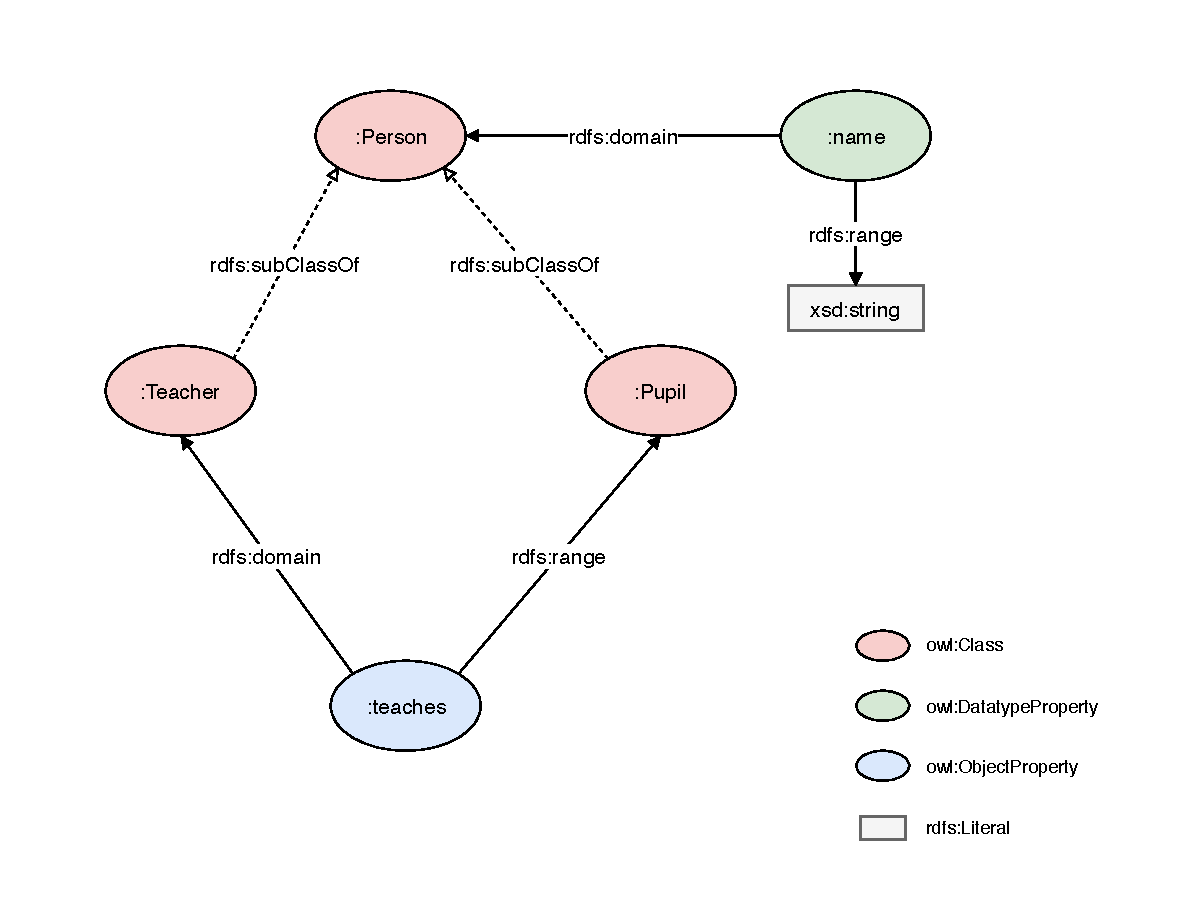
\includegraphics[width=\textwidth]{drawio/University_Ontology_Example}
	 \caption{Simple Ontology Graph}\label{fig:simple_owl_graph}
\end{figure}
For example, if the concept \textit{:Teacher} is taken as reference node, it makes sense to not only include the concept itself, but instead connected nodes~(e.g. the concept \textit{:Person} and the object property \textit{:teaches}) as well. 

As in the guidelines for conducting crowdsourcing research~\cite{sarasua2015crowdsourcing}, the authors recommended to avoid technical terms in crowdsourcing questions. In the next paragraphs we explain how \textit{ontology verbalisation} helps to achieve this goal. 

Despite the fact that natural language is desirable for descriptions as everybody knows and understands with no extra learning effort, it conflicts in terms of expressiveness and specificity with well defined ontologies which can encode complex data and relations in domain-specific areas. To resolve this conflict, a new language variant named \textbf{ACE}~\textit{(Attempto Controlled English)}~\cite{fuchs2008} was created. ACE is a formal language, capable of expressing domain-specific knowledge with a well defined syntax, supporting formal reasoning and readable by specialists who are yet unfamiliar with formal languages and methods.

To get a better understanding of ACE\footnote{\url{https://tinyurl.com/yc3zhu9a} accessed 2018/05/05}\footnote{\url{https://tinyurl.com/ycst39jv} accessed 2018/05/05}, a short overview of its language structure is given in the next paragraphs:
 
\paragraph{Simple Sentences} A Simple Sentence derived from standard English language contains a subject, a verb and additional elements: \texttt{subject + verb + complements [ + adjuncts ]} The verb relates direct or indirect to one or more other objects~(\textit{complements}). Optionally, to add more specificity, one or more adverbs and prepositional phrases can be added~(\textit{adjuncts}). 

\paragraph{Composite Sentences} A Composite Sentence is composed of one or more Simple~Sentences, connected by \textit{coordination},
\textit{subordination}, \textit{quantification} and \textit{negation}. Whereas coordination links sentences either by the word \texttt{and} or \texttt{or}, subordination relates dependent sentences in some way~(e.g. if-then sentences). Quantification allows statements about all~(universal quantification) or certain~(existential quantification) objects of a certain domain. Last, encoding negative polarity in a sentence~(e.g. sentences containing \texttt{not} or \texttt{no}) is defined as negation. 

\paragraph{Query Sentences} Query Sentences can be divided into polar questions~(e.g. with \textit{yes/no} answer) and non-polar questions, also known as \emph{wh-questions}. In contrast to yes/no questions no pre-defined answer exist for these. Furthermore, wh-questions start with either of the following five W-words: \texttt{Who}, \texttt{What}, \texttt{When}, \texttt{Where} and \texttt{Why}. However, this definition somewhat less strict as sometimes questions starting with the word \texttt{How} are included as well.

\paragraph{Anaphoric References} If the meaning of a word or phrase is context dependent, recurring occurrences of these expressions are called \textit{Anaphoric References}. More specifically, the referring term~(\textit{anaphor}) relates to an antecedent expression. For example, given the sentence: \texttt{Tom arrived, but nobody noticed him}, the pronoun \texttt{him} relates to \texttt{Tom}. To resolve ambiguities during the processing phase, Anaphoric References are replaced by encoded references. 

\textbf{OWL Verbalizer}~\cite{stevens2011}, an open source tool aimed at producing texts from generic OWL ontologies, is a good example of a successful integration of ACE. A description of the basic concepts of OWL Verbaliser is given below:

This tool, being now part of the \textbf{SWAT Tool Suite}\footnote{\url{http://mcs.open.ac.uk/nlg/SWAT/} accessed 2018/05/06}, was created to overcome the burden of maintaining ontology definitions by hand. Whereas producing high quality texts in restricted application domains is under active research, this tool produces understandable descriptions using general-purpose methods that are of moderate quality.

The high-level process of ontology verbalisation shown in \hyperref[fig:verbaliser_architecture]{Figure~\ref*{fig:verbaliser_architecture}} consists of the following stages:

\paragraph{Transcoding from OWL to Prolog} The output of this stage is a file in a convenient Prolog format which was generated from an ontology in RDF/XML format. The conversation process covered by the \textit{Transcoder}, \textit{Identifier~Selector} and \textit{Label~Selector} combines identifiers~(concepts, individuals, object~properties) and labels. In addition, ambiguous terms in identifiers are normalised. 

\paragraph{Constructing a lexicon for atomic entities} The output of this stage, covered by the component \textit{Lexicon Generator}, is a collection of lexicons, computed from the normalised Prolog terms in the previous stage. A lexical entry~(lexicon) is defined as a quadruple having the following form: \texttt{<identifier, part-of-speech, singular-form, plural-form>} To facilitate processing in later stages, normalised identifiers for concepts, individuals and object~properties are stored together with word category, singular form and plural form. The word~category, also known as part-of-speech, groups words based on similar properties in terms of syntax and grammar. Common categories are nouns, verbs and adjectives. Last, to differentiate the quantity of a phrase or word, singular and plural form of a noun are associated with each lexical entry. 
Among the storage of lexicons, the algorithm also implements other rules regarding text processing. Some simple heuristics are used for pre-processing to transform the resulting word string into better readable English sentences. 

\paragraph{Selecting the axioms relevant for describing each class} This stage and the next stage are covered by the \textit{Planner}.
This component has as input all axioms from the source ontology as well as the lexicons from the previous stage. In this stage, axioms are mapped to matching lexical entries. As matching criteria the algorithm uses the lexicon identifier and the IRI~\cite{rfc3987}. 

\paragraph{Aggregating axioms with a similar structure} This stage is optional, as it is not strictly required for text generation which is described in the next stage. However, some improvements are achieved if similar axioms are aligned. 

\paragraph{Generating sentences from axioms} The final stage is covered by the component named \textit{Realiser} which forms the central part of the
verbalisation process. English sentences are generated for each axiom using logical rules for almost every logical pattern in OWL-DL. These rules are expressed in Prolog clauses, taking the axiom and optionally the lexicon as input.

\begin{figure}
	 \centering
	 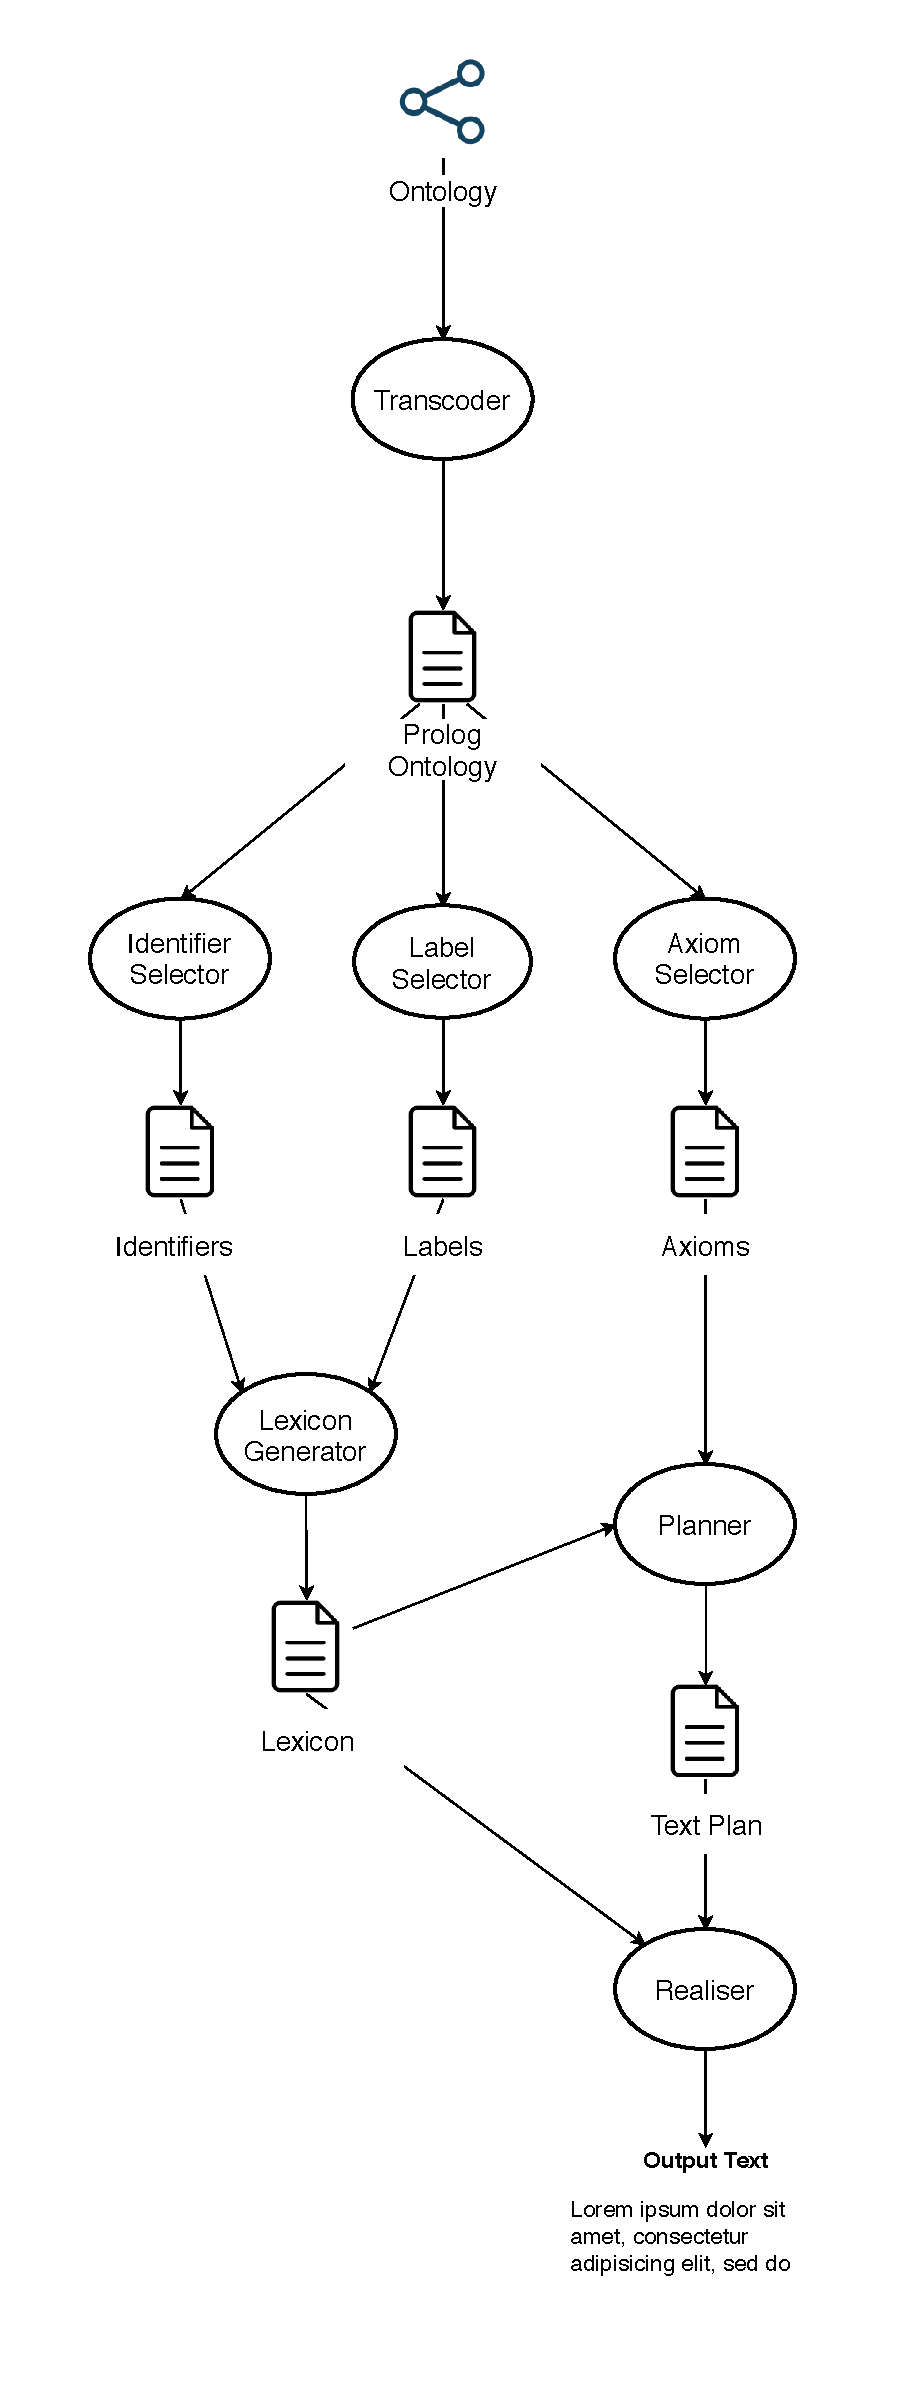
\includegraphics[width=0.5\textwidth]{drawio/Ontology_Verbaliser_Architecture}
	 \caption{Conceptual architecture of the OWL ontology verbaliser~\cite{stevens2011}}\label{fig:verbaliser_architecture}
\end{figure}

Although OWL~Verbaliser would be useful to integrate in the enrichment process, there are some major obstacles:

The first is \textbf{incompatibility on a language level}. Traditionally, software systems are written in many different programming languages, leading to the challenge of dealing with interoperability~\cite{malone2014}. While OWL~Verbaliser was written in SWI-Prolog, Protege runs on the Java Virtual Machine~(JVM), causing a conceptual mismatch in programming languages and paradigms. Moreover, interoperability between conceptually different programming languages is challenging in its own\footnote{\url{http://www.swi-prolog.org/packages/jpl/} accessed 2018/05/11} and would conflict with the goal of an easy-to-integrate solution.

Another obstacle is a \textbf{mismatch on the scope of operation}. OWL~Verbaliser was implemented as a tool assisting engineers in ontology creation, a very time consuming task. It was designed as a standalone tool, launched from the command line or deployed as a web service. On the other hand, ontology enrichment is embedded in Protege and part of the ontology validation process, operating only on small parts of the ontology. In contrast, OWL~Verbaliser takes the whole ontology as input. 

\paragraph{Proposed Approach for Ontology Validation} Due to this complicating issues, we implemented a different approach using some insights from OWL~Verbaliser. The pseudocode of the overall workflow is given in \hyperref[alg:neighbourhood]{Algorithm~\ref*{alg:neighbourhood}}. The notation to describe properties and relations is based on a formal Ontology~Description Logic~(DL)~\cite{baader2003}, string manipulations were formally defined in~\cite{hopcroft1969}.

\begin{algorithm}
	\caption{Context Enrichment based on Neighbouring Nodes}\label{alg:neighbourhood}
	\begin{algorithmic}[1]
		\Procedure{Generate Description}{}\newline
			\textbf{Input:} A concept $C$\newline
			\textbf{Output:} A textual description $T$ of $C's$ neighbouring nodes based on subsumption\newline
			\State{$T=\{\}$} \label{alg:neighbourhood:text_initialisation}
			\For {$ (c,d) \in C \sqsubseteq D $}
				\State $T=T$ $\cup$ "Every " $\cup$ $name(c)$ $\cup$ " is a " $\cup$ $name(d)$
			\EndFor
			\For {$ (e,c) \in E \sqsubseteq C $}
				\State $T=T$ $\cup$ "Every " $\cup$ $name(e)$ $\cup$ " is a " $\cup$ $name(c)$
			\EndFor
		\EndProcedure
	\end{algorithmic}
\end{algorithm}

The main work is done in two for-loops, which calculate context descriptions based on subsumption~$(\sqsubseteq)$ and string concatenation~$(\cup)$. To handle the case of missing subsumption relations, the output text $T$ is initialised to an empty string~(\hyperref[alg:neighbourhood:text_initialisation]{Line~\ref*{alg:neighbourhood:text_initialisation}}). Next, for every subsumption relation having the input concept $C$ in its signature, either $C's$ name or the anchor node's name is appended first. For example, given the following subsumption relations $\{Car \sqsubseteq Vehicle, Cabrio \sqsubseteq Car\}$, the algorithm generates $T=\{$\textit{"Every Car is a Vehicle"}$,$ \textit{"Every Cabrio is a Car"}$\}$ under the assumption that \textit{Car} was chosen as anchor node.

\section{Embedded Context}\label{sec:embedded_context}
Over the years ontologies were used in many domain contexts, including general-purpose as well as highly specialised ones. Obviously, what separates good ontologies from poor ones is how well they are documented~\cite{daquin2012}. Studies~\cite{dutta2017} analysed various approaches of embedding meta-data in ontologies. The outcome was that there is no standard way to describe and document ontologies, albeit a few vocabularies that describe semantic meta-data exist. 

In this section we give an overview of these approaches and explain in detail how we used that for ontology validation. In the remainder of this section our focus lies on semantic meta-data in the context of ontology engineering. A broader discussion on the use of meta-data in general is given in~\cite{nilsson2010}. 

\paragraph{Dublin Core~(DC)} Being one of the most prominent vocabulary in describing semantic meta-data, published and maintained by the Dublin Core Metadata Initiative~(DCMI), it originally contained 15 meta-data terms\footnote{\url{http://www.dublincore.org/documents/dces/} accessed 2018/05/20},  designed to annotate resources with simple, textual information. Since its first launch, the project have gained popularity, including more than 127 terms\footnote{\url{http://www.dublincore.org/documents/dcmi-terms/} accessed 2018/05/20}. The initial set of terms is listed in~\hyperref[table:dublin_core]{Table~\ref*{table:dublin_core}}. 

\begingroup
\renewcommand{\arraystretch}{2}
\begin{table}
	\begin{tabularx}{\textwidth}{l|X}
		\textbf{Name} & \textbf{Description} \\
		\hline
		\texttt{dc:contributor} & Element used to describe a person, organisation or service who is responsible for making contributions.\\
		\texttt{dc:overage} & Term used to describe a temporal topic~(e.g. period, date, or date range), spatial topic~(e.g. location or place identified by its name or coordnates) or a jurisdiction~(e.g. an administrative entity). \\
		\texttt{dc:creator} & A person, organisation or service who created this entity.\\
		\texttt{dc:date} & A period or point in time associated with an event in the lifecycle.\\
		\texttt{dc:description} & A definition in natural-language.\\
		\texttt{dc:format} & Defines the file format, physical medium or dimension.\\
		\texttt{dc:identifier} & A unique and unambiguous reference to this entity within a defined context.\\
		\texttt{dc:language} & The language used to describe and define this entity.\\
		\texttt{dc:publisher} & A person, organisation or service who provides access to this entity.\\
		\texttt{dc:relation} & Defines a link to another entity identified by name or formal identifier.\\
		\texttt{dc:rights} & A statement about associated rights with the entity~(e.g. intellectual property rights).\\
		\texttt{dc:source} & A related entity from which this entity is derived from.\\
		\texttt{dc:subject} & The topic of this entity represented using keywords, key-phrases or classification codes.\\
		\texttt{dc:title} & The name by which this entity is formally known.\\
		\texttt{dc:type} & Defines the genre of nature. Usually, a well-defined vocabulary such as DCMI Type Vocabulary\footnote{\url{http://dublincore.org/documents/dcmi-type-vocabulary/}} is recommended here.\\
	\end{tabularx}
	\caption{The initial set of DC-Metadata terms}
	\label{table:dublin_core}
\end{table}
\endgroup

To maximise interoperability in heterogeneous environments, an RDF-Schema with DCMI-Metadata\footnote{\url{http://dublincore.org/schemas/rdfs/} accessed 2018/05/20} elements was created, in which each entity is identified by a Uniform Resource Identifier~(URI) starting with the prefix \emph{http://purl.org}. 

\paragraph{Simple Knowledge Organisation~(SKOS)} The SKOS Core Vocabulary~\cite{skos2005} defines a set of RDF properties and RDFS classes
used to express the content and structure of a concept scheme, which describes sets of concepts with optionally linked concepts. The vocabulary is standardised by the W3C~Consortium\footnote{\url{https://www.w3.org/TR/skos-reference/} accessed 2018/05/20}. Relevant terms are listed in~\hyperref[table:skos]{Table~\ref*{table:skos}}.

\begingroup
\renewcommand{\arraystretch}{2}
\begin{table}
	\begin{tabularx}{\textwidth}{l|X}
		\textbf{Name} & \textbf{Description} \\
		\hline
		\texttt{skos:Concept} & Describes an idea, notion or unit of thought, similar to OWL classes. However the specification does draw any relations to \textit{owl:concept}.\\
		\texttt{skos:ConceptScheme} & A Concept Scheme can be viewed as a combination of multiple \textit{skos:Concept} instances with optional references to each other.\\
		\texttt{skos:altLabel} & A \textit{lexical label}~(e.g. a text composed of unicode characters) which adds an alternative meaning to an entity. \\
		\texttt{skos:prefLabel} & Used in combination with \textit{skos:altLabel} to define the primary description in case there are multiple human-readable definitions.\\
		\texttt{skos:notation} & A literal string of unicode characters, it identifies the related concept within the given concept scheme.\\
		\texttt{skos:changeNote} & Belongs to the class of \textit{documentation properties} and provides some information about historical changes.\\
		\texttt{skos:definition} & Adds a human-readable definition to the entity.\\
		\texttt{skos:note} & Some arbitrary text which may be provided by ontology engineers.\\
		\texttt{skos:editorialNote} & A note added by creators to inform ontology maintainers.\\
		\texttt{skos:historyNote} & A historical note~(e.g. a version string, release date, \ldots ).\\
        \texttt{skos:related} & Indicates that SKOS concepts are somewhat related to each other.\\
	\end{tabularx}
	\caption{A subset of the SKOS vocabulary}
	\label{table:skos}
\end{table}
\endgroup

There is some overlap between DC and SKOS. For example, the terms \textit{dc:subject} and \textit{skos:subject} describes similar characteristics of an entity. However, in some usage scenarios the range of skos:subject is limited to resources of type skos:concept compared to the unrestricted range of dc:subject. Moreover, in case there is more than one subject, the property \textit{skos:primarySubject} allows assertions of the entities or resources main subject. 

\paragraph{Open Biomedical Ontology~(OBO)} Biomedical systems are inherently complex and process large amounts of data. Managing these is
expensive and often requires expert knowledge. The Open Biomedical Ontologies~(OBO)~Foundry\footnote{\url{http://obofoundry.org/} accessed 2018/05/21}, a community of experienced ontology developers and engineers for biomedical environments, manages many specialised biomedical ontologies. These are available in various formats, including the OBO~format, which was originally developed as part of the Gene Ontology~(GO)\footnote{\url{http://www.geneontology.org/} accessed 2018/05/21}. 

The OBO File Format Specification~1.2~\footnote{\url{https://owlcollab.github.io/oboformat/doc/GO.format.obo-1_2.html} accessed 2018/05/22} defines a flat document structure for OBO files. A file contains a header and one or more \emph{stanzas}. A stanza is a labeled section of a document, indicating that an object of a particular type is being described. Currently, there are three supported types: \textit{Term}, \textit{Typedef} and \textit{Instance}. Every stanza starts with an id-tag and an unbounded list of tag-value pairs. Looking at the supported tags, it is clear that the definition of meta-data is important to achieve the goals of \textit{readability}, \textit{ease of parsing}, \textit{extensibility} and \textit{minimal redundancy}. In particular, it allows, among others, the specification of 
\begin{inparaenum}[1)]
		\item the term definition (\texttt{def}),
		\item comments (\texttt{comment}),
		\item editorial data~(\texttt{is\_obsolete}, \texttt{replaced\_by}, \texttt{created\_by}, \texttt{creation\_date}) and
		\item cross references (\texttt{xref})
\end{inparaenum}.

Although the Open Biomedical Ontologies and the Semantic Web have overlapping objectives, they evolved independently. To bring these two communities together, researchers have created a tool for converting OBO~ontologies to OWL and vice-versa without loosing any information during the conversion process~\cite{tirmizi2011}. It turned out that the majority of the OBO~vocabulary fits nicely into the Semantic Web Layer Cake. The mapping between the OBO Layer Cake and the Semantic Web Layer Cake is shown in~\hyperref[fig:semantic_obo_cake]{Figure~\ref*{fig:semantic_obo_cake}}. 

\begin{figure}
	 \centering
	 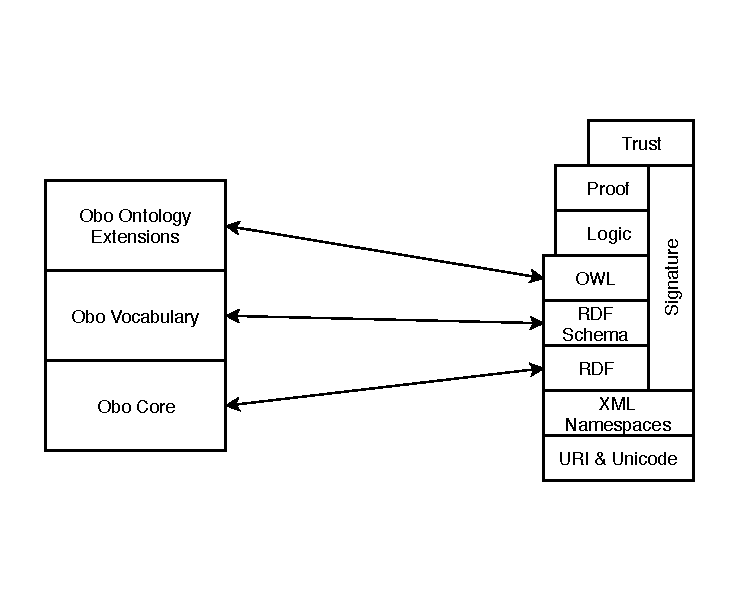
\includegraphics[width=0.5\textwidth]{drawio/Obo2Owl}
	 \caption{Mapping between OBO and the Semantic Web (depicted from~\cite{tirmizi2011})}\label{fig:semantic_obo_cake}
\end{figure}

\emph{OBO~Core} forms the bottom layer of the OBO Layer Cake. It mainly handles the assignment of ids and namespaces to RDF related concepts. Historically, OBO identifiers were limited in scope (local identifiers) while OWL requires global identifiers (URIs). This imposes some challenges on the translation process, e.g. URIs need to be prepended with prefixes. 

The next layer represents the \emph{OBO Vocabulary} which is mapped to RDF-Schema. As there exists a replacement for each of the terms in RDF-Schema, the translation process is implemented by replacing \texttt{names} with RDFS labels, \texttt{definitions} with RDFS labels, \texttt{comments} with RDFS comments, \texttt{is\_a} with subclass relations, \texttt{domains} with RDFS domain restrictions and \texttt{ranges} with RDFS range restrictions. 

The top most layer is represented by the \emph{OBO Ontology Extensions} which are mapped to OWL. Besides the definition of concept-level mappings, this layer defines tags for expressing meta-data on the entire ontology. For example, editorial meta-data (\texttt{creation\_date}, \texttt{replaced\_by} and \texttt{saved\_by}) is mapped to annotation properties. 

A summary of the most important OBO tags together with their OWL equivalents is given in~\hyperref[table:obo]{Table~\ref*{table:obo}}. However, for some OBO vocabulary there is no corresponding OWL tag. Therefore, a dedicated OWL namespace\footnote{http://www.geneontology.org/formats/oboInOwl\#} containing all OBO definitions was created. Furthermore, a recommended practice to preserve compatibility between OBO features and OWL features is to restrict editing of mapped OBO tags. A more detailed discussion on this topic is given in~\cite{tirmizi2011, tirmizi2006}.

\begingroup
\renewcommand{\arraystretch}{2}
\begin{table}
	\begin{tabularx}{\textwidth}{l|l|X}
		\textbf{Name} & \textbf{OWL Translation} & \textbf{Description} \\
		\hline
        \texttt{obo:def} & oboInOwl:Definition & The definition of the term in natural language.\\
		\texttt{obo:synonym} & oboInOwl:Synonym & An indication that there exists a tag with the same meaning.\\
		\texttt{obo:comment} & rdfs:comment & A remark to the term. \\
		\texttt{obo:xref} & oboInOwl:DbXref & A reference to an analogous term in another vocabulary.\\
		\texttt{obo:date} & oboInOwl:hasDate & The creation or modification date.\\
		\texttt{obo:saved-by} & oboInOwl:savedBy & The username of the person who edited the file last.\\
		\texttt{obo:replaced\_by} & oboInOwl:replacedBy & A reference to a newer term which replaces the obsolete one.\\
	\end{tabularx}
	\caption{A subset of the OBO vocabulary used as meta-data}
	\label{table:obo}
\end{table}
\endgroup

\paragraph{Proposed Approach for Ontology Validation} Given the high number on ontology meta-data formats from above, \hyperref[alg:embedded_enrichment]{Algorithm~\ref*{alg:embedded_enrichment}} shows the pseudocode to create concept descriptions extracted from embedded meta-data. In addition to the notation used in the previous section we define $\Phi(C) \coloneqq \{m_1, m_2, \ldots, m_i \}$ where $m_i$ is the $i'th$ meta-data element embedded in concept $C$ and $T$ is the description of some meta-data element.

\begin{algorithm}
	\caption{Context Enrichment based on embedded meta-data}\label{alg:embedded_enrichment}
	\begin{algorithmic}[1]
		\Procedure{Generate Description}{}\newline
			\textbf{Input:} A concept $C$ with embedded meta-data $\{m_1, m_2, \ldots, m_i \}$\newline
			\textbf{Output:} A description $T$ of $C's$ meta-data elements\newline
			\State{$T=\{\}$}
			\For {$ m_k \in \Phi(C) $}
				\State $T=T$ $\cup$ $m_k$
			\EndFor
		\EndProcedure
	\end{algorithmic}
\end{algorithm}

While the actual enrichment is straightforward, it collects all descriptions for a determined concept, the details of extracting the meta-data from annotation properties is omitted here because it highly depends on the chosen meta-data encoding.
As we decided to encode the meta-data in annotation properties, the extraction process works by selecting the related annotation properties for a specified concept. 

\section{External Source}\label{sec:external_source}
An alternative method of context enrichment is based on fetching concept definitions from external sources. The lookup is solely based on the concept's name, neglecting the connected nature of an ontology. Dictionaries have always been the first choice when it comes to searching for specific information about words or phrases.

This section begins with an introduction in the theory of dictionaries, discusses searching problems and strategies to overcome these and briefly describes several online dictionaries including the one we used in our approach.

\paragraph{Short Introduction into Lexicography}
Dictionaries, as most humans are familiar with, contain the \textit{lexicon} of a language, that is a collection of words or phrases, called the lexemes. 
They are designed for word lookups and facilitate finding information about spelling, meaning and usage. Historically, written dictionaries were constrained by the alphabetised format and once printed, never updated. On the other hand, online dictionaries facilitate accessing the information on more than one path, semantics being one of them. Similarly, keeping the word up-to-date as well as adding new ones is as simple as updating or adding new records to the database, compared to printing and distributing new copies of their written pedants. 

Lexicography is defined as the science about~\enquote{the theory and practice of dictionaries, that is, dictionaries, encyclopaedias, lexica, glossaries, vocabularies, terminological knowledge bases, and other information tools covering areas of knowledge and its corresponding language.}~\cite{fuertes2017}
Among other definitions, they share the understanding that lexicography is an interdisciplinary science with characteristics of linguistic science, information science and others. 

When it comes to classifying electronic dictionaries, it is obvious that they are more than just machine-readable copies of their printed counterparts, but rather comprehensive software conglomerates only limited by technological, economical and/or practical constraints. The key defining elements of electronic dictionaries are 
\begin{inparaenum}[i)]
		\item the access principle,
		\item the construction principle and
		\item the distinction between information databases and information tools
\end{inparaenum}~\cite{fuertes2011}.
Whereas the \textit{access principle} deals with providing quick and easy access to the needed information, the \textit{construction principle} differentiates dictionaries based on the technical and economical aspects when building the dictionary. Special attention should be paid to the division between information databases and information tools, that is, separating user concerns~(searching and viewing the results) from the underlying data organisation. 

Depending on the usage scenarios, several types of dictionaries have emerged over the years. A recent study~\cite{mueller_spitzer2013} evaluated, how dictionaries are being used or, in other words, the external conditions or situations in which a dictionary consultation is embedded.  
In their research, participants with professional and academic background were asked about the circumstances of dictionary usage. 
Analyses revealed that responses can be partitioned into the following \textit{groups of usage} situations: 
\begin{enumerate}
	\item Text Production
	\item Text Reception
	\item Text Translation
\end{enumerate}

\textit{Text Production} is the action of writing texts in professional or personal contexts. Dictionary content vary in many ways, depending on writer's profession and text category. For example, passive speech using domain specific vocabularies are dominant in academic literature over active speech and simple language constructs in short-term, informal texts~\cite{o2010routledge}~(e.g. emails, tweets, Facebook posts, \ldots).

\textit{Text Reception} is the process or theory that emphasises the meaning and interpretation of existing literature. Readers focus on writing reviews and understanding texts. The user's motivation of dictionary interaction is finding the word definition as well as looking for samples~(e.g. example sentences), synonyms/antonyms and links to external information. 

\textit{Text Translation} is the process of converting text from a source language to a target language by preserving its meaning. Unfortunately there is not always a one-to-one mapping possible because of lacking equivalent language constructs in the target language. Old-fashioned dictionaries containing translations for specific words do not help either because words are lacking context. With the advent of online dictionaries, new opportunities for translators appeared such as spelling correction and links to synonyms/antonyms. Not only professional translators responded that dictionaries are crucial for their business, students and teachers consult dictionaries to improve their vocabulary, look up pronunciation or simply find the contexts of word usage. 

\paragraph{Searching in Electronic Dictionaries} Searching is probably the most important feature of today's electronic dictionaries. In the next paragraphs we discuss problems that arise when searching for specific terms and strategies to overcome these. 

Several studies~\cite{pastor2010, mvechura2008} have analysed digital dictionaries, available in different languages and accessible via the Internet or compressed on a digital medium~(e.g. CD-ROM). Their evaluation is based on empirical analyses of user behaviour collected from log-files as well as literature review. All searching techniques listed below tackle the problem of invalid, incomplete, misspelled and multi-word search queries.

The first category are \textit{inflection-aware} search algorithms which accept inflected and uninflected search queries. The central part of these algorithms are rewrite rules which transform the input query to the matching headword or vice-versa. A powerful but complicated technique is based on a deep understanding of the target language. It is based on morphologies of the word endings. For example, stripping \emph{-ed} and \emph{-ing} endings for regular verbs is yet simple but only manageable for regular verbs, more complicated algorithms are needed for irregular verbs. Other algorithms, not taking the structure of the target language into account, are based on fuzzy string searching, a technique based on approximate string matching. A simple metric measuring the difference between two strings is the Levenshtein~Distance~\cite{levenshtein1966}. It is defined as the number of single character manipulations necessary to transform one string into the other. 

The next category are algorithms dealing with \textit{multi-word} search items. Search algorithms need to deal with user entered search strings, containing multiple words or even complete sentences. The situation is even more complicated, for a single-word search query users expect not only matching single-word entries but also matching multi-word entries~(e.g. phrasal verb). Enumerating all possible word combinations might be acceptable in dictionaries with small corpora, but it is infeasible in dictionaries with millions of entries and performance is important. In these cases it is better to construct an index from single-word entries and multi-word entries. An even better approach, also known by the term \emph{lemmatising}, would be to analyse and process the words before-hand.

Another challenge in processing search queries is \textit{detecting misspellings}. User input is inherently prone to errors. Smart algorithms guide the user to the intended word by offering corrections and suggestions, similar to what a spellchecker does. A naive approach would be to collect lists of common misspelled words and continue with matching. This has the disadvantage that not all possible combinations are included and processing takes longer, especially for long word lists. A better but yet more complicated technique is based on word similarity which is discussed in the previous paragraph. 

A technique especially useful for multi-lingual dictionaries is \textit{language selection and detection}. As there already exists much literature in this area~\cite{mcnamee2005, lodhi2002, vatanen2010, selamat2016}, we decided to just outline two approaches here. The first group of algorithms is purely based on statistical models. The detection of the target language works by building probabilistic models of the inferred statistics and the pre-trained statistics. The second group works by counting common words or character sequences~(called n-grams) and comparing the obtained frequency counts against reference values~\cite{mcnamee2005}.

The last technique is \textit{text normalisation}. It solves the problem of unwanted characters in search strings by removing variation and reducing words to simpler formats. For search strings, this means that noisy characters are removed. A simple strategy is to delete characters which do not add any meaning such as hyphens, dots quotation marks and (mathematical)~symbols. Additionally, consecutive occurrences of whitespaces are merged. 
The normaliser also need to consider some character variations as defined by the Unicode~Standard\footnote{\url{http://www.unicode.org/reports/tr15/} accessed 2018/06/08 }. 

\paragraph{Online Dictionary Examples} We have chosen some well-known, freely accessible online dictionaries that were used in various research
fields.

%WordNet
Started as a research project in 1985 at Princeton University \textbf{WordNet}~\cite{fellbaum1998} is best characterised as a dictionary browser rather than just an online dictionary. It allows users to explore its contents on the basis of semantic, rather than alphabetic similarities. Users look up information along more than one path, semantics being among them. How one wants to explore the possibilities of online dictionaries rather depends on one's ideas and applications one has in mind. 

The building blocks of WordNet are \textit{synsets} which are defined as sets of words having similar semantics~(synonymy). It is important that synonymy does not entail unrestricted interchangeability. By that criterion natural languages would have very few synonyms. Instead, synonymy is typically relative to a context which is encoded as links between and within synsets. 
Several linguistic relations are defined in WordNet, for example \textit{polysemy/monosemy}, \textit{hyponymy/hypernymy} and \textit{meronymy/holonymy}. 
Polysemy/Monosemy describes the fact that a word may have multiple meanings or one meaning. Hyponymy/Hypernymy means that words or phrases are included in the meaning of another word. Meronymy/Holonymy describes part-of or member-of relationships.

The WordNet architecture~\cite{fellbaum1998} as illustrated in~\hyperref[fig:wordnet_architecture]{Figure~\ref*{fig:wordnet_architecture}} can be split into these parts:
\begin{enumerate}
		\item Lexical Source Files
		\item the Grinder
		\item the Lexical Database
		\item Software Tools and Interfaces
\end{enumerate}

\begin{figure}
	 \centering
	 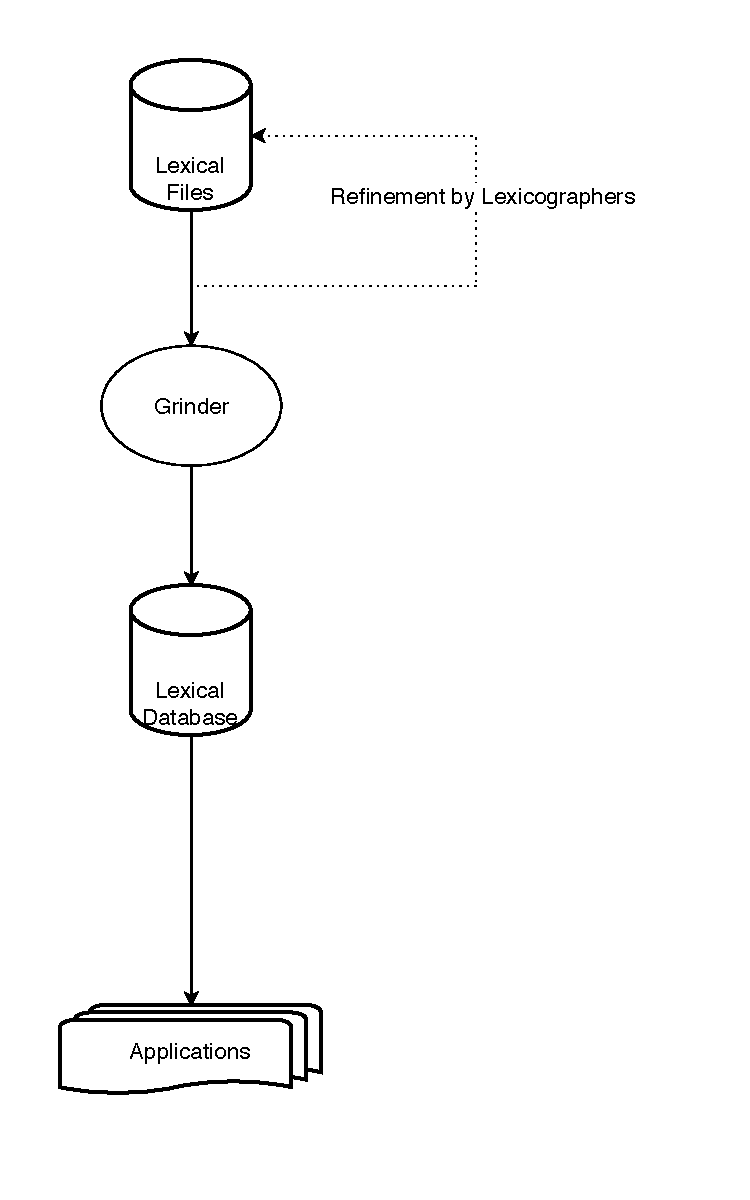
\includegraphics[width=0.5\textwidth]{drawio/WordNet_Architecture}
	 \caption{The architecture of the WordNet System~\cite{fellbaum1998}}\label{fig:wordnet_architecture}
\end{figure}


The \textit{Lexical Database} forms the heart of the WordNet system. It is the result of processing all lexical source files. There are many tools available, written in various programming languages like Perl or awk, to interact with the database. 

WordNet offers some \textit{interfaces} to users for interaction. Depending on the area of application there are textual interfaces~(Command Line Interfaces and APIs) and graphical interfaces~(Desktop Software and Web Applications). Invoking the search form and starting search tasks can also be done via browser interface\footnote{\url{http://wordnetweb.princeton.edu/perl/webwn} accessed 2018/06/14}.

WordNet's key success factor is its potentials in terms of Natural Language Processing~(NLP). It was also used as information source in many other fields~\cite{morato2004}, these are: Image Retrieval, Information Retrieval, Document Classification, Query Expansion, Machine Translation and Conceptual Disambiguation.

A different approach was taken by \textbf{WordNik}\footnote{\url{https://www.wordnik.com/} accessed 2018/06/15}. It targets native English speakers who look up words that are rare~(technical terms or dialect terms), very old or very new. They often search for definitional information which is incomplete or missing in traditional dictionaries. Users tolerate published imperfection because they opt for relevant, actual and cutting-edge information, even though not officially approved by editors~\cite{burnett1979}. They want to understand the context of word usage in sentences, not necessarily explanatory statements as in printed or even online dictionaries.

The driving force behind WordNik was contribution. It processes and aggregates external user-generated content such as tweets, newspaper articles, scientific articles or uploaded Flickr\footnote{\url{https://www.flickr.com/} accessed 2018/06/15} images. This is similar to what search engines do, but with restricted scope. The creators of WordNik observed that very few people write word definitions, they rather add meta linguistic information such as lists of their favourite words, comments or tags. WordNik additionally collects statistics about lexicographical terms, more or less frequently searched words and most commented words. 

WordNik also offers an API for programmatically accessing their resources\footnote{\url{https://developer.wordnik.com/} accessed 2018/06/15}. At the time of writing this thesis free access is granted for non-profit, non-commercial use with a limitation on the number of API calls. 
After a successful registration process, an API token is provided which is a prerequisite for API interaction. Besides Web access, a handful of libraries\footnote{\url{https://developer.wordnik.com/libraries} accessed 2018/06/15}, available in many programming languages, were created to facilitate integration with third-party applications. 

\textbf{Wiktionary}\footnote{\url{https://www.wiktionary.org/} accessed 2018/06/15} is a freely accessible, collaborative online lexicon~\cite{granger2012}. Whereas traditional dictionaries are the product of a small group of expert lexicographers, collaboratively constructed dictionaries are created by many, not necessarily expert users. This has the advantage that new lexical entries are added more frequently and existing ones are continuously updated. Users are encouraged to participate in content creation and maintenance. New lexical entries are discussed in the community until a consensus is reached. 

An important goal of Wiktionary is openness towards multilingualism. It was first launched in 2002 and indented as an "add-on" to Wikipedia\footnote{\url{https://www.wikipedia.org/} accessed 2018/06/16}. At that time it was only available in English, but now translations exist for nearly every spoken language. However, they differ in scope and community size. Each Wiktionary is accessible by prepending the respective ISO~639~language~code\footnote{\url{https://www.iso.org/iso-639-language-codes.html} accessed 2018/06/16} to the common wiktionary domain.

Content is organised as collections of pages, each containing a title and a body. There are four page categories:
\begin{inparaenum}[1)]
		\item Article Pages,
		\item Redirect Pages,
		\item Talk Pages and
		\item Internal Pages
\end{inparaenum}.
Most pages are \emph{Article Pages}, containing the actual linguistic information. With \emph{Redirect Pages}, users are able to navigate from page to page. At page creation, \emph{Talk Pages} help editors in collecting ideas, expressing criticism, asking questions and discussing page contents. \emph{Internal Pages} are protected and contain motivational information, goals, statistics, indices, appendices and guidelines for contributors. 

Wiktionary is not targeted to specific groups of people nor its content serves a specific purpose, instead, it is open for everyone. 
Linguistic knowledge is organised in separate sections as explained in the next paragraphs: 

It may sound surprising that each page starts with the \emph{language} of the term or phrase because each page belongs to a specific translation of Wiktionary anyway. However, this is necessary because the same term can be encoded in multiple languages. For example, the term \texttt{boat} is used in five languages\footnote{\url{https://en.wiktionary.org/wiki/boat} accessed 2018/06/16}. 

The \textit{etymology} section describes origin and history of a word. It helps linguists in exploring linguistic relations such as synonymy/antonymy, hypernymy/hyponymy and homonymy/polysemy. They are also interested, whether and how the meaning has changed over time. 

\textit{Phonetic references} are appreciated not only by language learners but also by readers who are unfamiliar with particular terms. The term's pronunciation is encoded using audio samples or phonetic notations. 

In contrast to other dictionaries which focus on canonical word forms, Wiktionary also contains entries for inflected word forms. For example, the English verb \texttt{go} and its \textit{morphology} \texttt{went} are encoded as separate entries. Additionally, it may include the declension of an adjective or the conjunction of a verb.

Each term is associated with a \textit{syntactic category} which includes part of speech tags for single words, idioms, proverbs and multi-word expressions. Apart from these, there are also other tags available. For example, nouns are marked as countable/uncountable or singular/plural. 

The most interesting part for dictionary readers is probably the section \textit{semantic knowledge} which describes the meaning of a term. It includes example sentences, quotations, links to other terms, glosses and linguistic labels. The gloss of a word is either a marginal or interlinear notation of the word's meaning. Non-linguists are eventually more familiar with the term \emph{glossary} which denotes to collections of glosses. 

\textit{Cross-lingual knowledge} is especially important for translators and educators who are interested in multilingual realtions. This is expressed as links between pages of differing language. For example, descriptions of the English word \texttt{boat} are contained in a page with links to \texttt{water~craft}, \texttt{full-house} and conformation to \texttt{cyclohexane}.

A valuable feature for non-native speakers is \emph{graphical knowledge}. It is obvious that humans grasp the meaning of a term faster by just looking at a picture or photograph than reading through long textual descriptions. Unfortunately, not all terms can be expressed in pictures or photographs though. 

From a technical perspective Wiktionary is based on MediaWiki\footnote{\url{https://www.mediawiki.org/wiki/MediaWiki} accessed 2018/06/17}, a free and open source software written in PHP\footnote{\url{http://www.php.net/} accessed 2018/06/17}. The software is distributed under the GNU~General~Public~License~(GPL) and maintained by the WikiMedia~Foundation\footnote{\url{https://wikimediafoundation.org/wiki/Home} accessed 2018/06/17}, a non-profit organisation aimed at supporting free, multilingual, educational content. MediaWiki is also used by many other wikis\footnote{\url{https://wikistats.wmflabs.org/} accessed 2018/06/17}.

The majority of wiki features are accessible via public API. Clients can request features or send commands over the \textit{MediaWiki~Action~API}\footnote{\url{https://www.mediawiki.org/wiki/API:Main_page} accessed 2018/06/17}. It has querying, searching, parsing and manipulation capabilities.

\paragraph{Proposed Approach for Ontology Validation} Intuitively, the idea of generating descriptions using dictionary lookups is simple: starting from a concept name, descriptions are built from consulting an online dictionary. 

A schematic overview of the overall workflow is shown in~\hyperref[fig:external_source_workflow]{Figure~\ref*{fig:external_source_workflow}}.
\begin{figure}
	 \centering
	 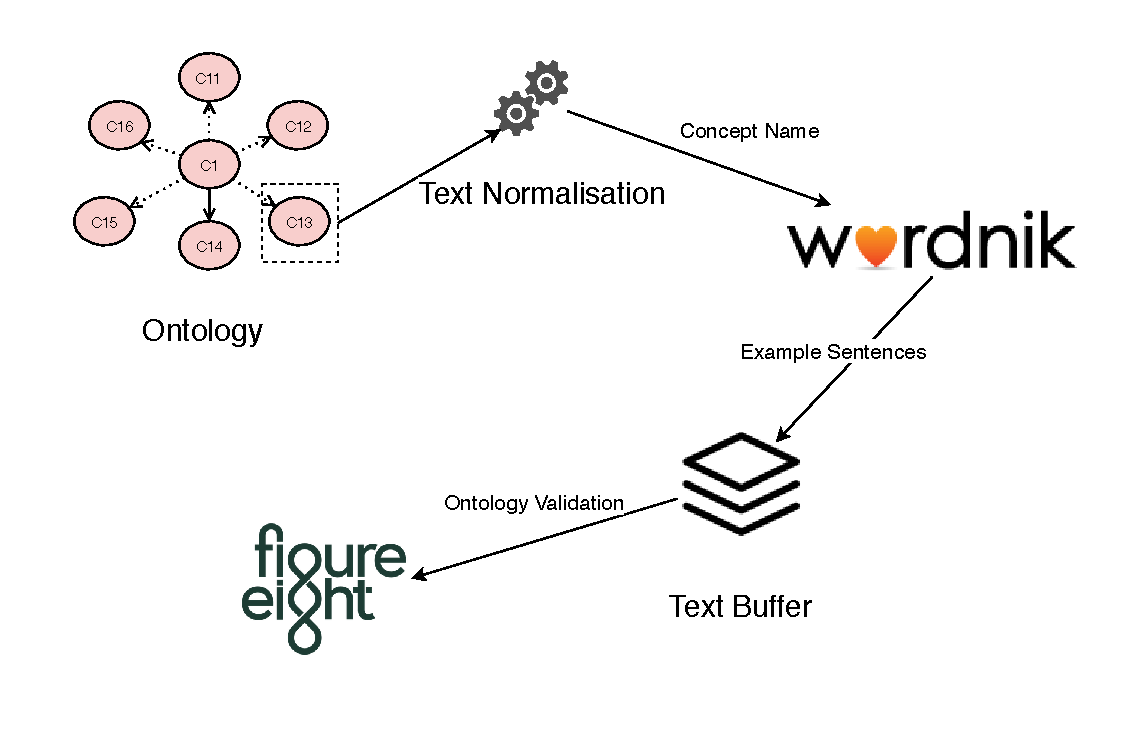
\includegraphics[width=0.9\textwidth]{drawio/External_Source_Workflow}
	 \caption{Conceptual workflow of WordNik consultation to generate concept descriptions}\label{fig:external_source_workflow}
\end{figure}
The idea is to use the concept name as a baseline for any further processing. Often, the name can not be used directly as input to WordNik because it contains unwanted characters such as excessive spaces, quotes, dots or just non-printable characters. This is especially true for learned ontologies, generated from textual sources. Our algorithm uses the built-in text manipulation capabilities of the JDK to pre-process concept names. Among the other approaches introduced earlier in this section, it is yet simple but still provides good results. 

Next, WordNik is consulted to find example sentences for normalised concept names. In contrast to traditional dictionaries, WordNik searches in all kinds of available online content, including newspapers, journals, scientific publications, tweets and others. 
All API interaction is protected against unauthorised access, however, to help developers learning the API, some features are available in isolated Sandbox~Mode\footnote{\url{https://developer.wordnik.com/docs} accessed  2018/06/21}. For instance, example sentences for the word \texttt{bird} can be fetched from the URL \texttt{/word.json/bird/examples}.

Depending on wether a single concept or multiple concepts are validated, example sentences need to be harmonised, which is realised by storing intermediate results and mapping these to the initial concepts. 

To conclude, this approach is rather simple and easy to implement, however, it may have the potential to generate wrong results, especially for ambiguous concept names. 
